\documentclass[11pt,a4paper]{article}

% 宏包
\usepackage[margin=1in]{geometry} % 设置页边距
\usepackage[UTF8]{ctex}  % 支持中文
\usepackage{graphicx}
\usepackage{subcaption} % 替换 subfigure 为 subcaption
\usepackage{booktabs}
\usepackage{amsmath}
\usepackage{amssymb}
\usepackage{float}
\usepackage{cite}
\usepackage{caption}
\usepackage{hyperref} % 添加超链接支持

% 标题信息
\title{\textbf{Flow Matching 实验报告}}
\author{孙文辉,电子工程系,2025316110}
\date{\today}

\begin{document}

\maketitle


\section{引言}
\label{sec:introduction}

Flow Matching \cite{lipman2023flow}提出了一种新的生成建模框架，通过连续时间公式和最优传输（Optimal Transport, OT）路径，实现了更简单的训练过程和更高效的采样。具体而言，Flow Matching使用OT路径将噪声和数据通过直线连接，形成常数速度的向量场，使得ODE求解器可以使用更大的步长，从而在更少的NFE下达到相同的生成质量。

本文从0开始，复现了Flow Matching论文的核心实验，在2D Toy数据和CIFAR-10数据集上完整实现了三种方法：Flow Matching (OT路径)、Flow Matching (VP路径)和DDPM baseline，并通过NFE效率分析验证了OT路径的优势。
除了在无条件生成任务上的实验，我们还扩展实现了类别条件生成模型，进一步展示了Flow Matching在条件生成任务中的潜力。
\subsection{主要工作}
\begin{itemize}
\item \textbf{算法复现与系统对比}：在 2D Toy 和 CIFAR-10 数据集上完整复现了 Flow Matching (OT/VP 路径) 与 DDPM baseline。
\item \textbf{采样效率验证}：通过 NFE 效率分析验证了 OT 路径在低 NFE 下的显著优势，相比 DDPM 实现了数倍的加速。
\item \textbf{几何直觉分析}：通过可视化手段揭示了 OT 路径（直线）与扩散模型路径（曲线）在训练复杂度和采样稳定性上的差异。
\item \textbf{类别条件生成扩展}：实现了基于 Cross-Attention 机制的类别条件生成模型，展示了 Flow Matching 在条件生成任务中的有效性。
\end{itemize}

\section{相关工作与核心理论}
\label{sec:related_work}

\subsection{扩散模型与连续时间流}

传统的扩散模型（DDPM \cite{ho2020denoising}）通过模拟高斯扩散过程将数据转化为噪声。虽然其生成质量优秀，但受限于 SDE 框架的随机性，往往需要复杂的采样 schedule 和极高的采样步数。Score-Based Generative Models \cite{song2021score} 将其统一到连续时间框架下，揭示了概率流 ODE的存在。然而，训练此类模型通常需要处理难以求解的 score function 或在训练循环中通过昂贵的数值积分来计算似然。

\subsection{Flow Matching}

Flow Matching \cite{lipman2023flow} 的观点如下：既然知道噪声起点 $x_0$ 和数据终点 $x_1$，就可以直接构建一条理想路径，并让神经网络学习该路径上的\textbf{速度（或者说向量场）}

\textbf{1. 模拟 ODE 为回归向量场} \\
假设存在概率路径 $p_t(x)$，$t \in [0, 1]$，其中 $p_0$ 为高斯噪声，$p_1$ 为数据分布。该路径由向量场 $v_t(x)$ 驱动，遵循连续性方程。Flow Matching 的目标是训练网络 $v_\theta(t, x)$ 逼近真实向量场 $u_t(x)$。

\textbf{2. 条件流匹配 (CFM)} \\
由于全局边缘分布 $p_t(x)$ 对应的真实向量场 $u_t(x)$ 涉及全局混合信息而不可解，论文提出了 CFM 定理：
\begin{equation}
\mathcal{L}_{CFM}(\theta) = \mathbb{E}_{t, q(x_1), p_t(x|x_1)} \| v_\theta(t, x) - u_t(x|x_1) \|^2
\end{equation}
这意味着只需学习针对单个数据点 $x_1$ 的条件向量场 $u_t(x|x_1)$。定理证明，学好局部条件向量场等价于学好了全局边缘向量场，这使得损失函数退化为简单的均方误差（MSE）回归，无需在训练时解 ODE。从而大大简化了训练过程，提升了训练效率。

\textbf{3. 最优传输路径 (Optimal Transport Path)} \\
不同于扩散模型弯曲的路径，OT 路径在几何上是连接 $x_0$ 与 $x_1$ 的直线：
\begin{equation}
x_t = (1 - t)x_0 + t x_1 \implies u_t(x|x_1) = x_1 - x_0
\end{equation}
可以从以下几个方面理解 OT 路径的优势：
\begin{itemize}
    \item \textbf{路径是直的}：相比扩散模型的比较混乱的收敛方式，OT 路径更加直接。
    \item \textbf{速度恒定}：目标速度 $x_1 - x_0$ 不随时间变化，神经网络极易拟合。
    \item \textbf{推理极快}：由于轨迹平直，Euler 法等简单积分器在极低 NFE 下即可精确采样。
\end{itemize}

\section{方法实现}
\label{sec:method}

\subsection{模型实现}

本实验在两种规模的数据集上进行了验证：
\begin{itemize}
    \item \textbf{2D Toy 数据}：使用多层感知机（MLP）拟合向量场，模型输入包含空间坐标与时间步，通过 Sinusoidal Embedding 处理时间特征。
    \item \textbf{CIFAR-10 图像}：采用 U-Net 架构作为向量场预测网络。模型通过 Residual Blocks 与 Self-Attention 层提取空间特征，并使用 Skip Connections 保持多尺度信息。
\end{itemize}

\subsection{路径配置}

本实验对比了三种路径：
\begin{itemize}
    \item \textbf{OT (Optimal Transport)}：直线路径，向量场为 $x_1 - x_0$。
    \item \textbf{VP (Variance Preserving)}：基于三角函数的曲线路径，模拟扩散模型的演化轨迹。
    \item \textbf{DDPM (Baseline)}：传统加噪去噪路径，使用 DDIM 确定性采样进行推理。
\end{itemize}

\subsection{类别条件生成扩展 (扩展部分)}

为了进一步验证 Flow Matching 在条件生成任务中的表现，我们实现了基于类别标签的定向生成模型。

\begin{itemize}
    \item \textbf{Cross-Attention 机制}：在 U-Net 的中间层与采样层引入交叉注意力机制。将类别标签通过 Learnable Embedding 转化为条件向量，作为 Attention 的 Key 和 Value，而图像特征作为 Query，从而实现特征图对类别信息的自适应捕捉。
    \item \textbf{轻量化架构}：设计了 \texttt{UNetWithClassLabels} 模型，参数量约为 2.4M。该模型在保持生成质量的同时，通过特征融合（Additive Fusion）与注意力引导，实现了高效的条件控制。
\end{itemize}

\section{训练过程与演化分析}
\label{sec:training}

\subsection{损失函数收敛}

图 \ref{fig:train_loss} 展示了三种方法在 CIFAR-10 上的训练损失曲线，图像左侧为Loss，右侧为NLL。可以看到，所有方法均在 1000 epoch 内实现了平稳收敛。
相比 DDPM，基于 Flow Matching 的方法展现出更稳定的训练过程，基本在200 epoch 后损失趋于平稳，说明向量场回归的训练目标更易优化。


\begin{figure}[htbp]
\centering
\begin{subfigure}{0.32\textwidth}
    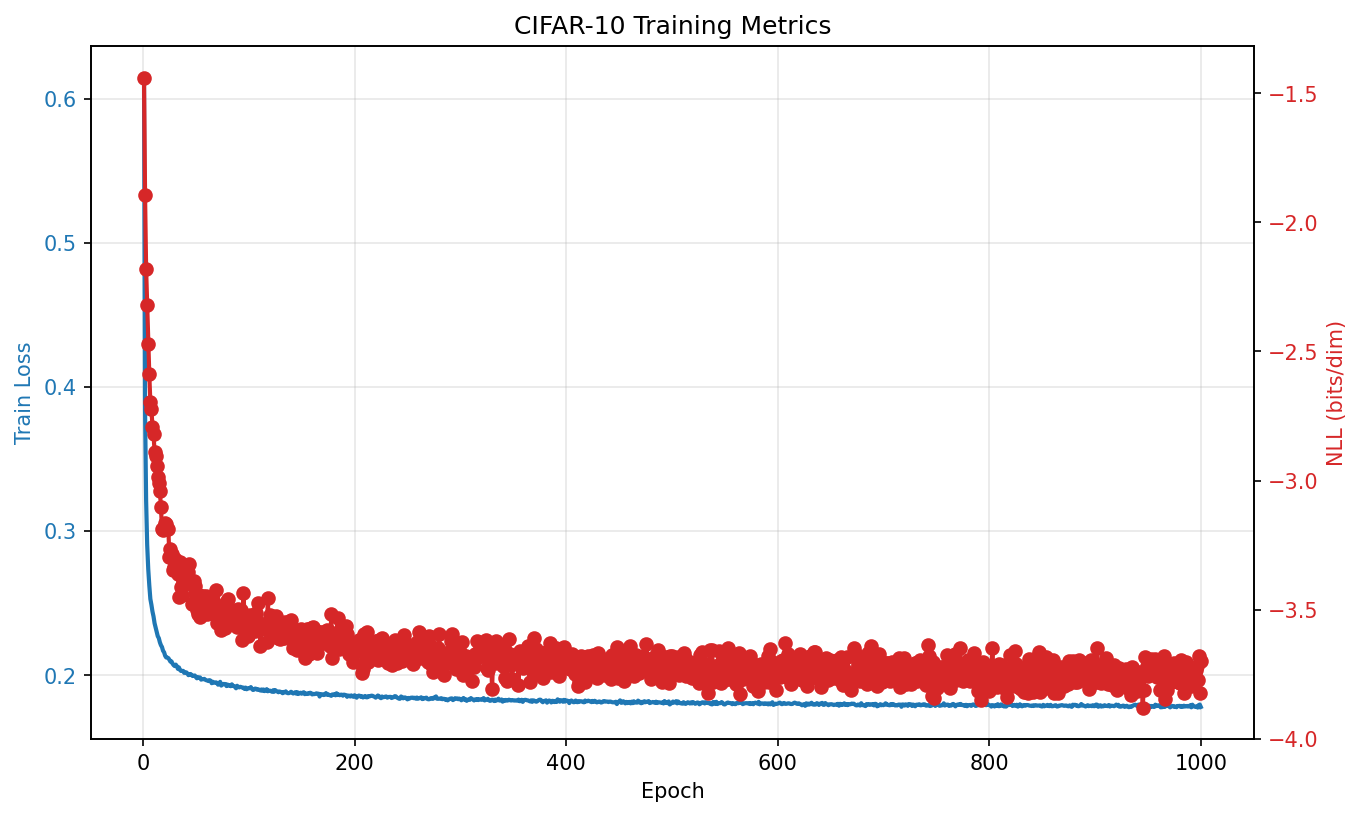
\includegraphics[width=\linewidth]{figures/cifar10/training/ot_loss.png}
    \caption{FM-OT Loss}
\end{subfigure}
\hfill
\begin{subfigure}{0.32\textwidth}
    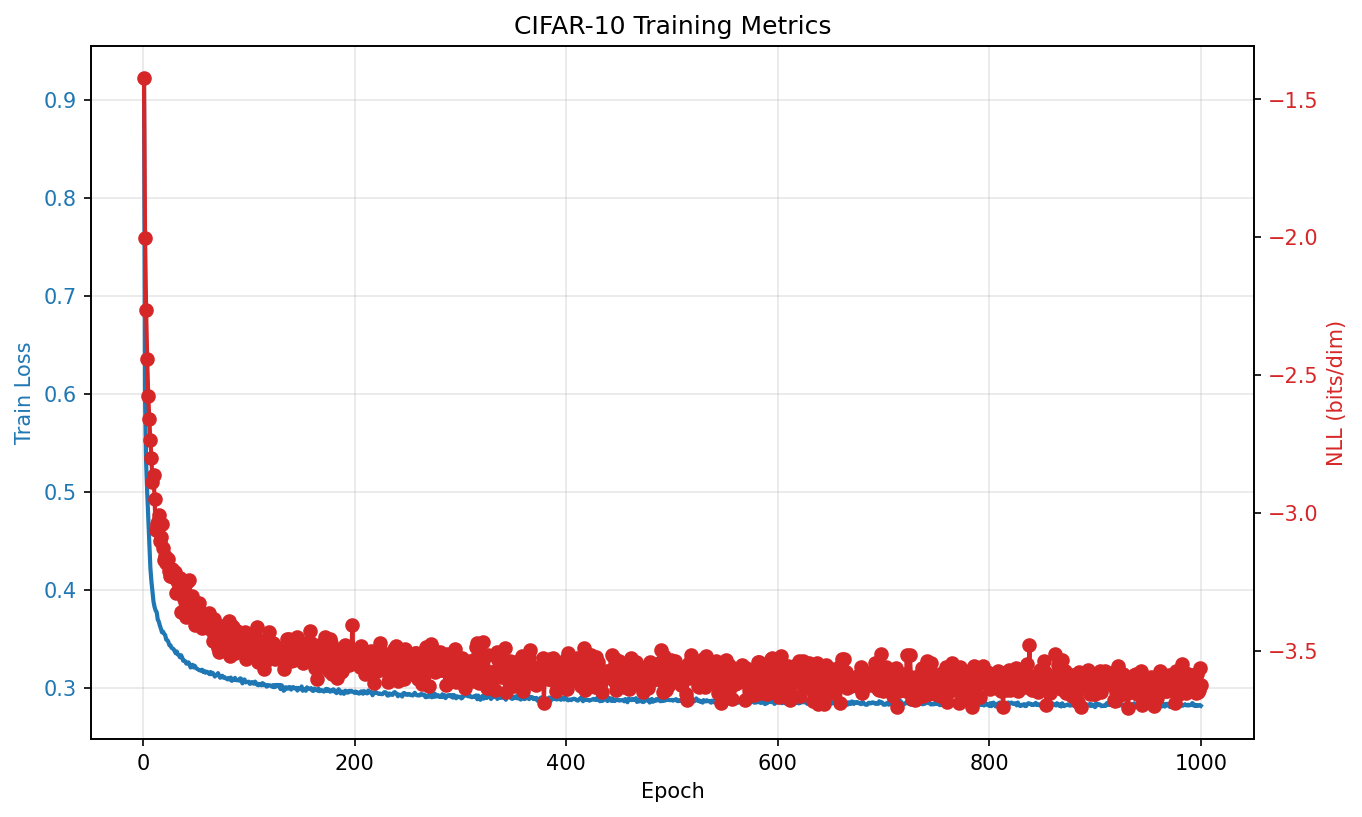
\includegraphics[width=\linewidth]{figures/cifar10/training/vp_loss.png}
    \caption{FM-VP Loss}
\end{subfigure}
\hfill
\begin{subfigure}{0.32\textwidth}
    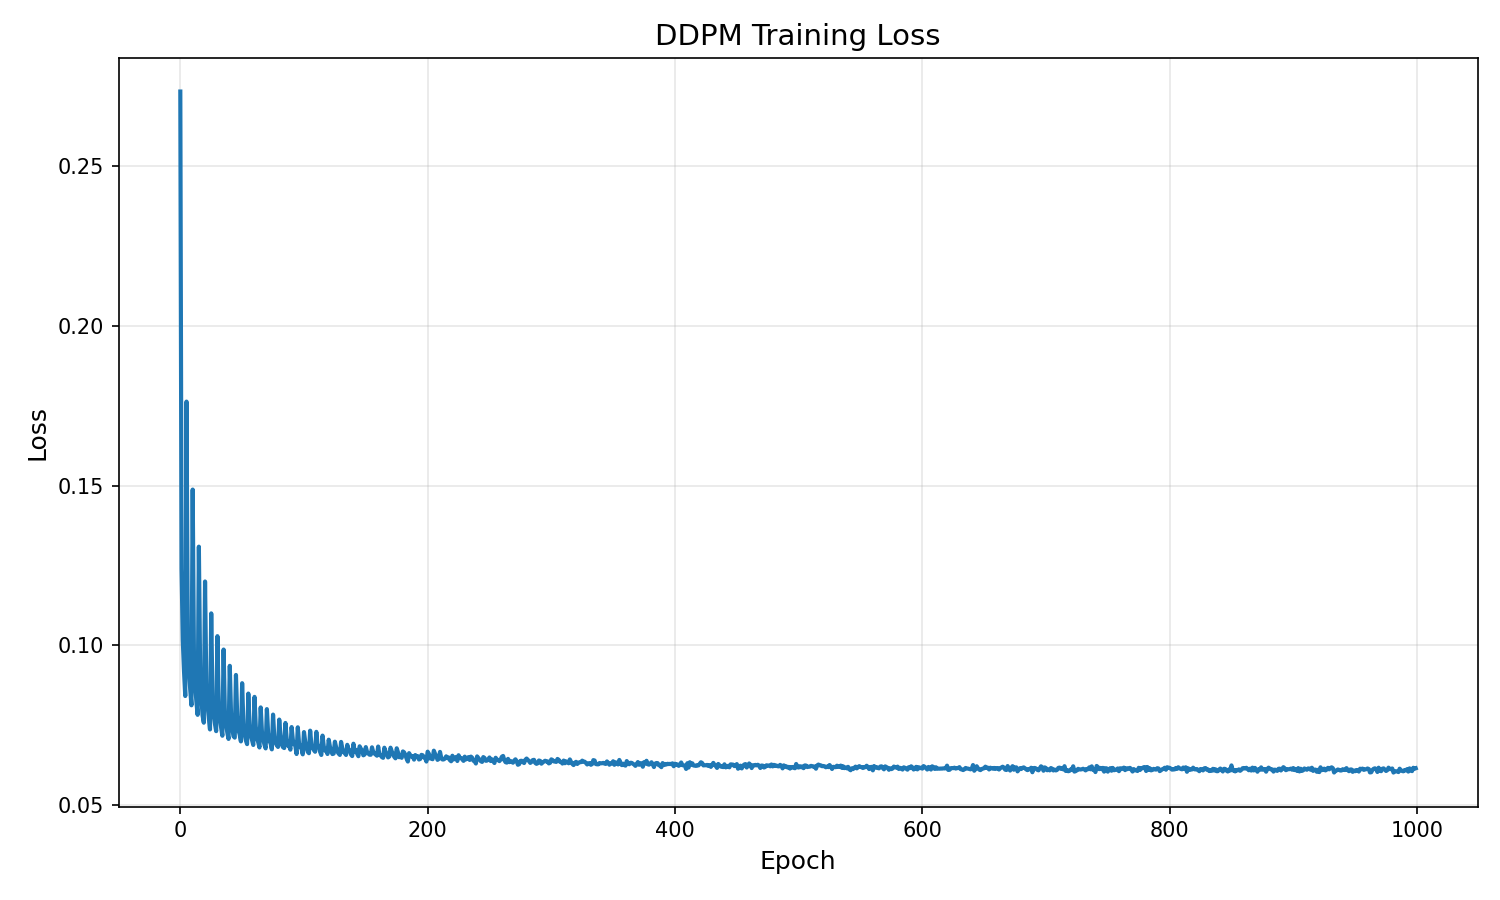
\includegraphics[width=\linewidth]{figures/cifar10/training/ddpm_loss.png}
    \caption{DDPM Loss}
\end{subfigure}
\caption{训练损失曲线对比。}
\label{fig:train_loss}
\end{figure}

\subsection{样本演化对比}

图 \ref{fig:sample_evolution} 展示了模型在训练过程中的生成能力演化。为了方便展示，我们选取了第 10, 20, 50, 100, 1000 epoch 的采样结果：

\begin{figure}[htbp]
\centering
\renewcommand{\arraystretch}{0.5}
\setlength{\tabcolsep}{1pt}
\begin{tabular}{cccccc}
& \textbf{Epoch 10} & \textbf{Epoch 20} & \textbf{Epoch 50} & \textbf{Epoch 100} & \textbf{Epoch 1000} \\
\rotatebox{90}{~~~\textbf{OT}} &
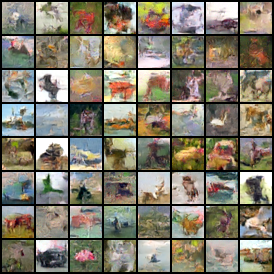
\includegraphics[width=0.18\textwidth]{figures/cifar10/training/ot_10.png} &
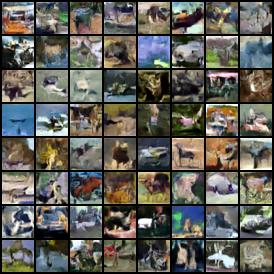
\includegraphics[width=0.18\textwidth]{figures/cifar10/training/ot_20.png} &
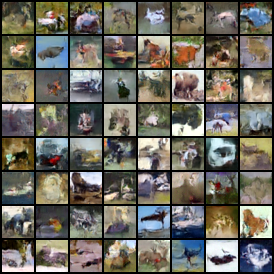
\includegraphics[width=0.18\textwidth]{figures/cifar10/training/ot_50.png} &
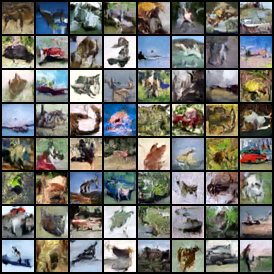
\includegraphics[width=0.18\textwidth]{figures/cifar10/training/ot_100.png} &
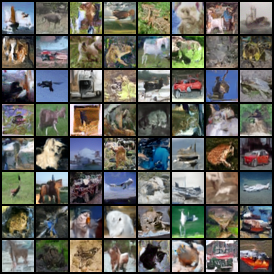
\includegraphics[width=0.18\textwidth]{figures/cifar10/training/ot_1000.png} \\
\rotatebox{90}{~~~\textbf{VP}} &
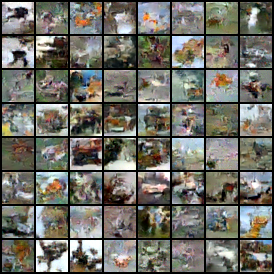
\includegraphics[width=0.18\textwidth]{figures/cifar10/training/vp_10.png} &
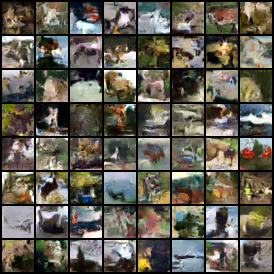
\includegraphics[width=0.18\textwidth]{figures/cifar10/training/vp_20.png} &
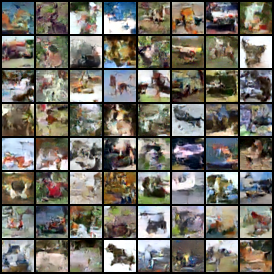
\includegraphics[width=0.18\textwidth]{figures/cifar10/training/vp_50.png} &
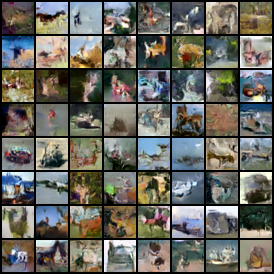
\includegraphics[width=0.18\textwidth]{figures/cifar10/training/vp_100.png} &
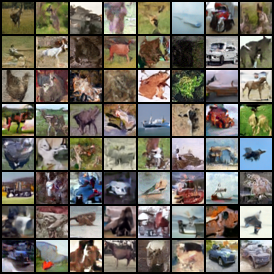
\includegraphics[width=0.18\textwidth]{figures/cifar10/training/vp_1000.png} \\
\rotatebox{90}{~~~\textbf{DDPM}} &
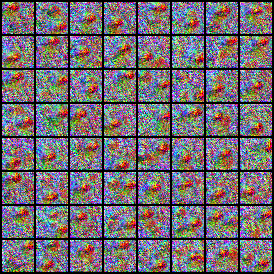
\includegraphics[width=0.18\textwidth]{figures/cifar10/training/ddpm_10.png} &
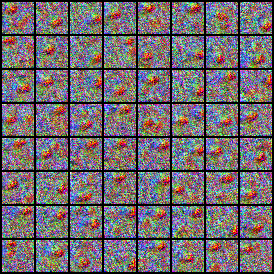
\includegraphics[width=0.18\textwidth]{figures/cifar10/training/ddpm_20.png} &
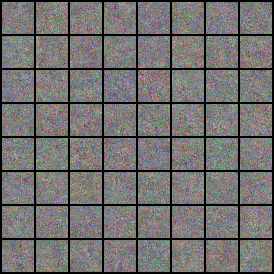
\includegraphics[width=0.18\textwidth]{figures/cifar10/training/ddpm_50.png} &
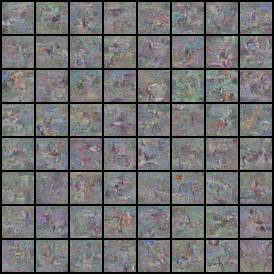
\includegraphics[width=0.18\textwidth]{figures/cifar10/training/ddpm_100.png} &
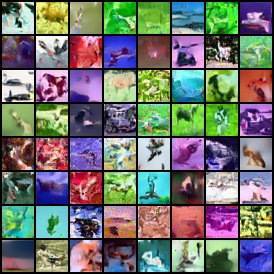
\includegraphics[width=0.18\textwidth]{figures/cifar10/training/ddpm_1000.png}
\end{tabular}
\caption{不同训练阶段的生成样本演化（NFE=100）。OT 路径在早期即可捕捉到清晰的物体轮廓，展现了强大的学习效率。}
\label{fig:sample_evolution}
\end{figure}

从图中可以看出，OT 路径在训练的前 10 个 epoch 内就表现出了比 DDPM 更强的结构建模能力。
DDPM的训练效果相对滞后，在实际测试过程中，DDPM即使在1000 epoch时也未能达到理想的生成质量，这
某种程度上与我们的采样步数设置的不合理有关，但实际上，为了保证实验的公平性，三种模型都是用相同的采样步数，在后文
对于FID的分析上也可以看出，基于Flow Matching的方法在低NFE下就能取得远超DDPM的效果。\\

\subsection{注：DDPM的实验过程}
由于没有复用现有的代码，全部模型都是从0开始的，加上期末周时间有限，跑一次完全的训练需要近5个小时，
所以DDPM的实验结果可能并没有达到最优，我对于这种巨大的差异也感到诧异，事实上，DDPM的现有结果
是在经过修正beta schedule错误（训练过程使用了“cosine”而在采样过程中使用了“linear”）后得到的，之前的结果更差。不过即使如此，Flow Matching的相对优势依然是显著的。
在训练完成后，我对最后的模型使用不同的NFE进行了采样，结果如下：
\begin{figure}[htbp]
\centering
\renewcommand{\arraystretch}{0.5}
\setlength{\tabcolsep}{1pt}
\begin{tabular}{cccccc}
& \textbf{NFE 10} & \textbf{NFE 100} & \textbf{NFE 200} & \textbf{NFE 300} & \textbf{NFE 1000} \\
\rotatebox{90}{~~~\textbf{DDPM}} &
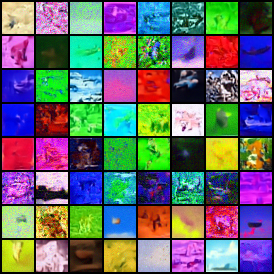
\includegraphics[width=0.18\textwidth]{figures/cifar10/training/samples_nfe10.png}&
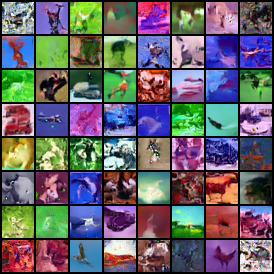
\includegraphics[width=0.18\textwidth]{figures/cifar10/training/samples_nfe100.png}&
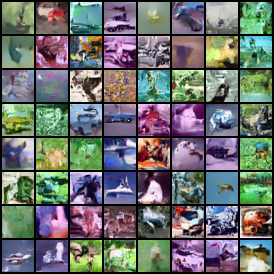
\includegraphics[width=0.18\textwidth]{figures/cifar10/training/samples_nfe200.png}&
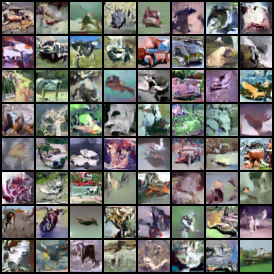
\includegraphics[width=0.18\textwidth]{figures/cifar10/training/samples_nfe300.png}&
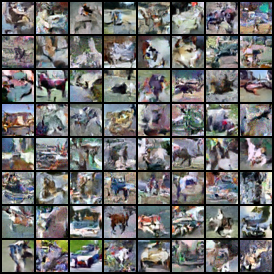
\includegraphics[width=0.18\textwidth]{figures/cifar10/training/samples_nfe1000.png}
\end{tabular}
\caption{1000epoch下DDPM在不同NFE下的结果}
\label{fig:DDPMatNFE}
\end{figure}
\\可以看到，在NFE步数足够的情况下，DDPM的生成效果有明显的改善。


\section{实验结果与效率评估}
\label{sec:results}

\subsection{2D Toy 数据：几何直觉验证}

为了直观体现 Flow Matching 的工作机制，我们在 2D Checkerboard 数据集上进行了详细的可视化分析。

\subsubsection{粒子演化动力学}

图 \ref{fig:toy_evolution} 纵向展示了 OT、VP 和 DDPM 三种方法从噪声 ($t=0$) 到数据 ($t=1$) 的演化过程。

\begin{figure}[htbp]
\centering
\begin{subfigure}{0.8\textwidth}
    \centering
    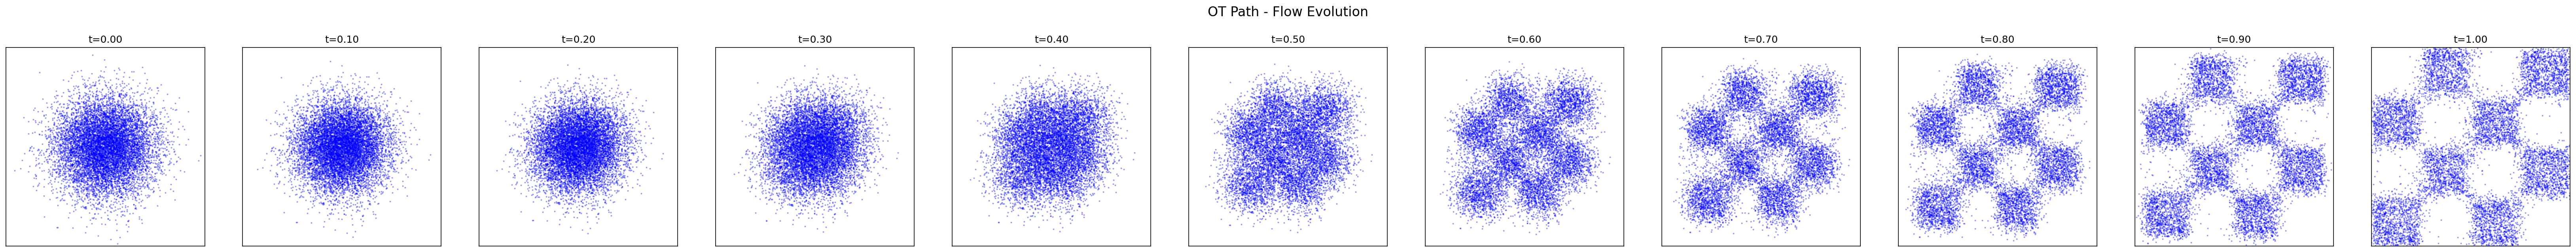
\includegraphics[width=\linewidth]{figures/toy/flow_evolution_OT.png}
    \caption{FM (OT) 演化：粒子沿直线迅速汇聚，中间状态 ($t=0.5$) 已具备较为清晰结构。}
\end{subfigure}
\\[2ex]
\begin{subfigure}{0.8\textwidth}
    \centering
    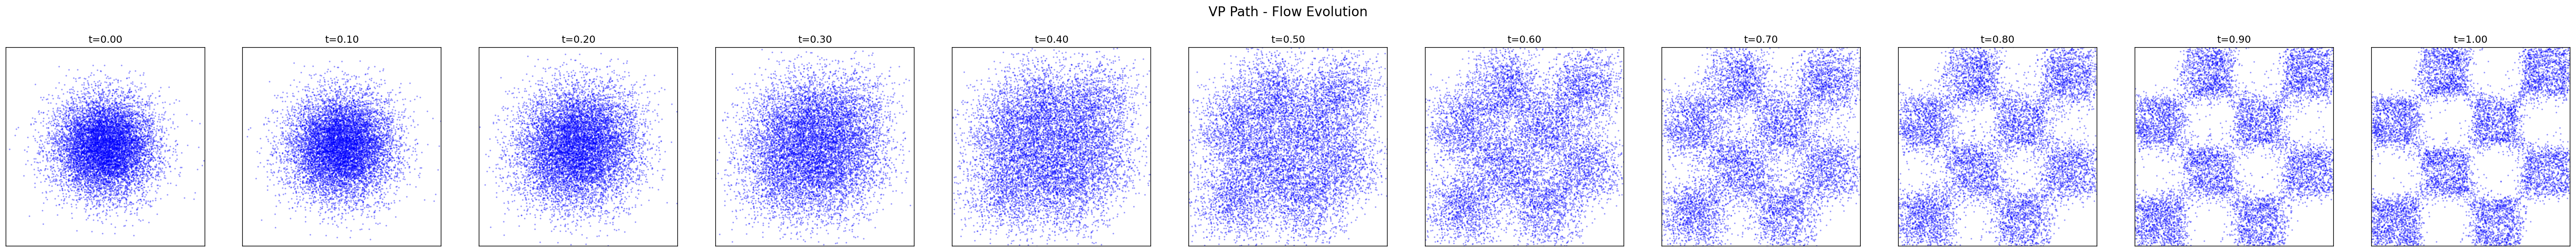
\includegraphics[width=\linewidth]{figures/toy/flow_evolution_VP.png}
    \caption{FM (VP) 演化：呈现出类似于扩散过程的曲线运动特征。}
\end{subfigure}
\\[2ex]
\begin{subfigure}{0.8\textwidth}
    \centering
    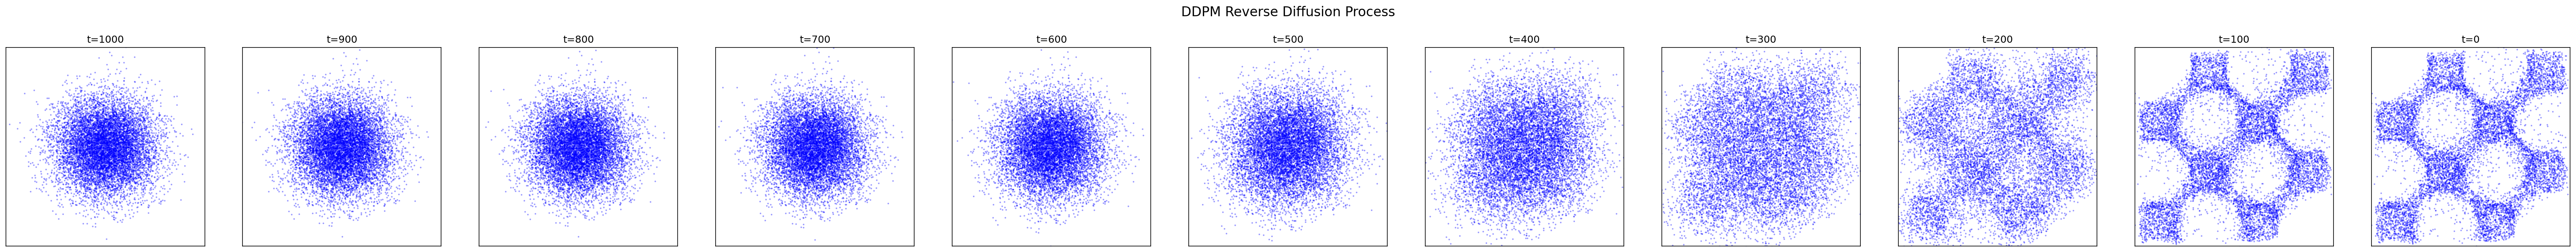
\includegraphics[width=\linewidth]{figures/toy/ddpm_evolution.png}
    \caption{DDPM 演化：演化动力学相对滞后，噪声消除过程较为缓慢。}
\end{subfigure}
\caption{2D Toy 粒子演化过程对比。}
\label{fig:toy_evolution}
\end{figure}

对比发现，OT 路径的粒子运动最具目的性，几乎没有冗余的布朗运动成分，在很短的时间内就能形成基本的结构轮廓
然后在简单的直线路径上完成微调，这一现象在后面的向量场上也能够体现。这种高效的运动方式解释了其在低 NFE 下的优越表现。相比之下，DDPM 展现出更复杂的运动轨迹，粒子在空间中经历了更多的迂回和扩散过程，导致采样效率降低。

\subsubsection{轨迹与向量场分析}

进一步地，我们分析了微观层面的生成轨迹与向量场特性（图 \ref{fig:toy_mechanisms}）。

\begin{figure}[htbp]
\centering
\begin{subfigure}{0.6\textwidth}
    \centering
    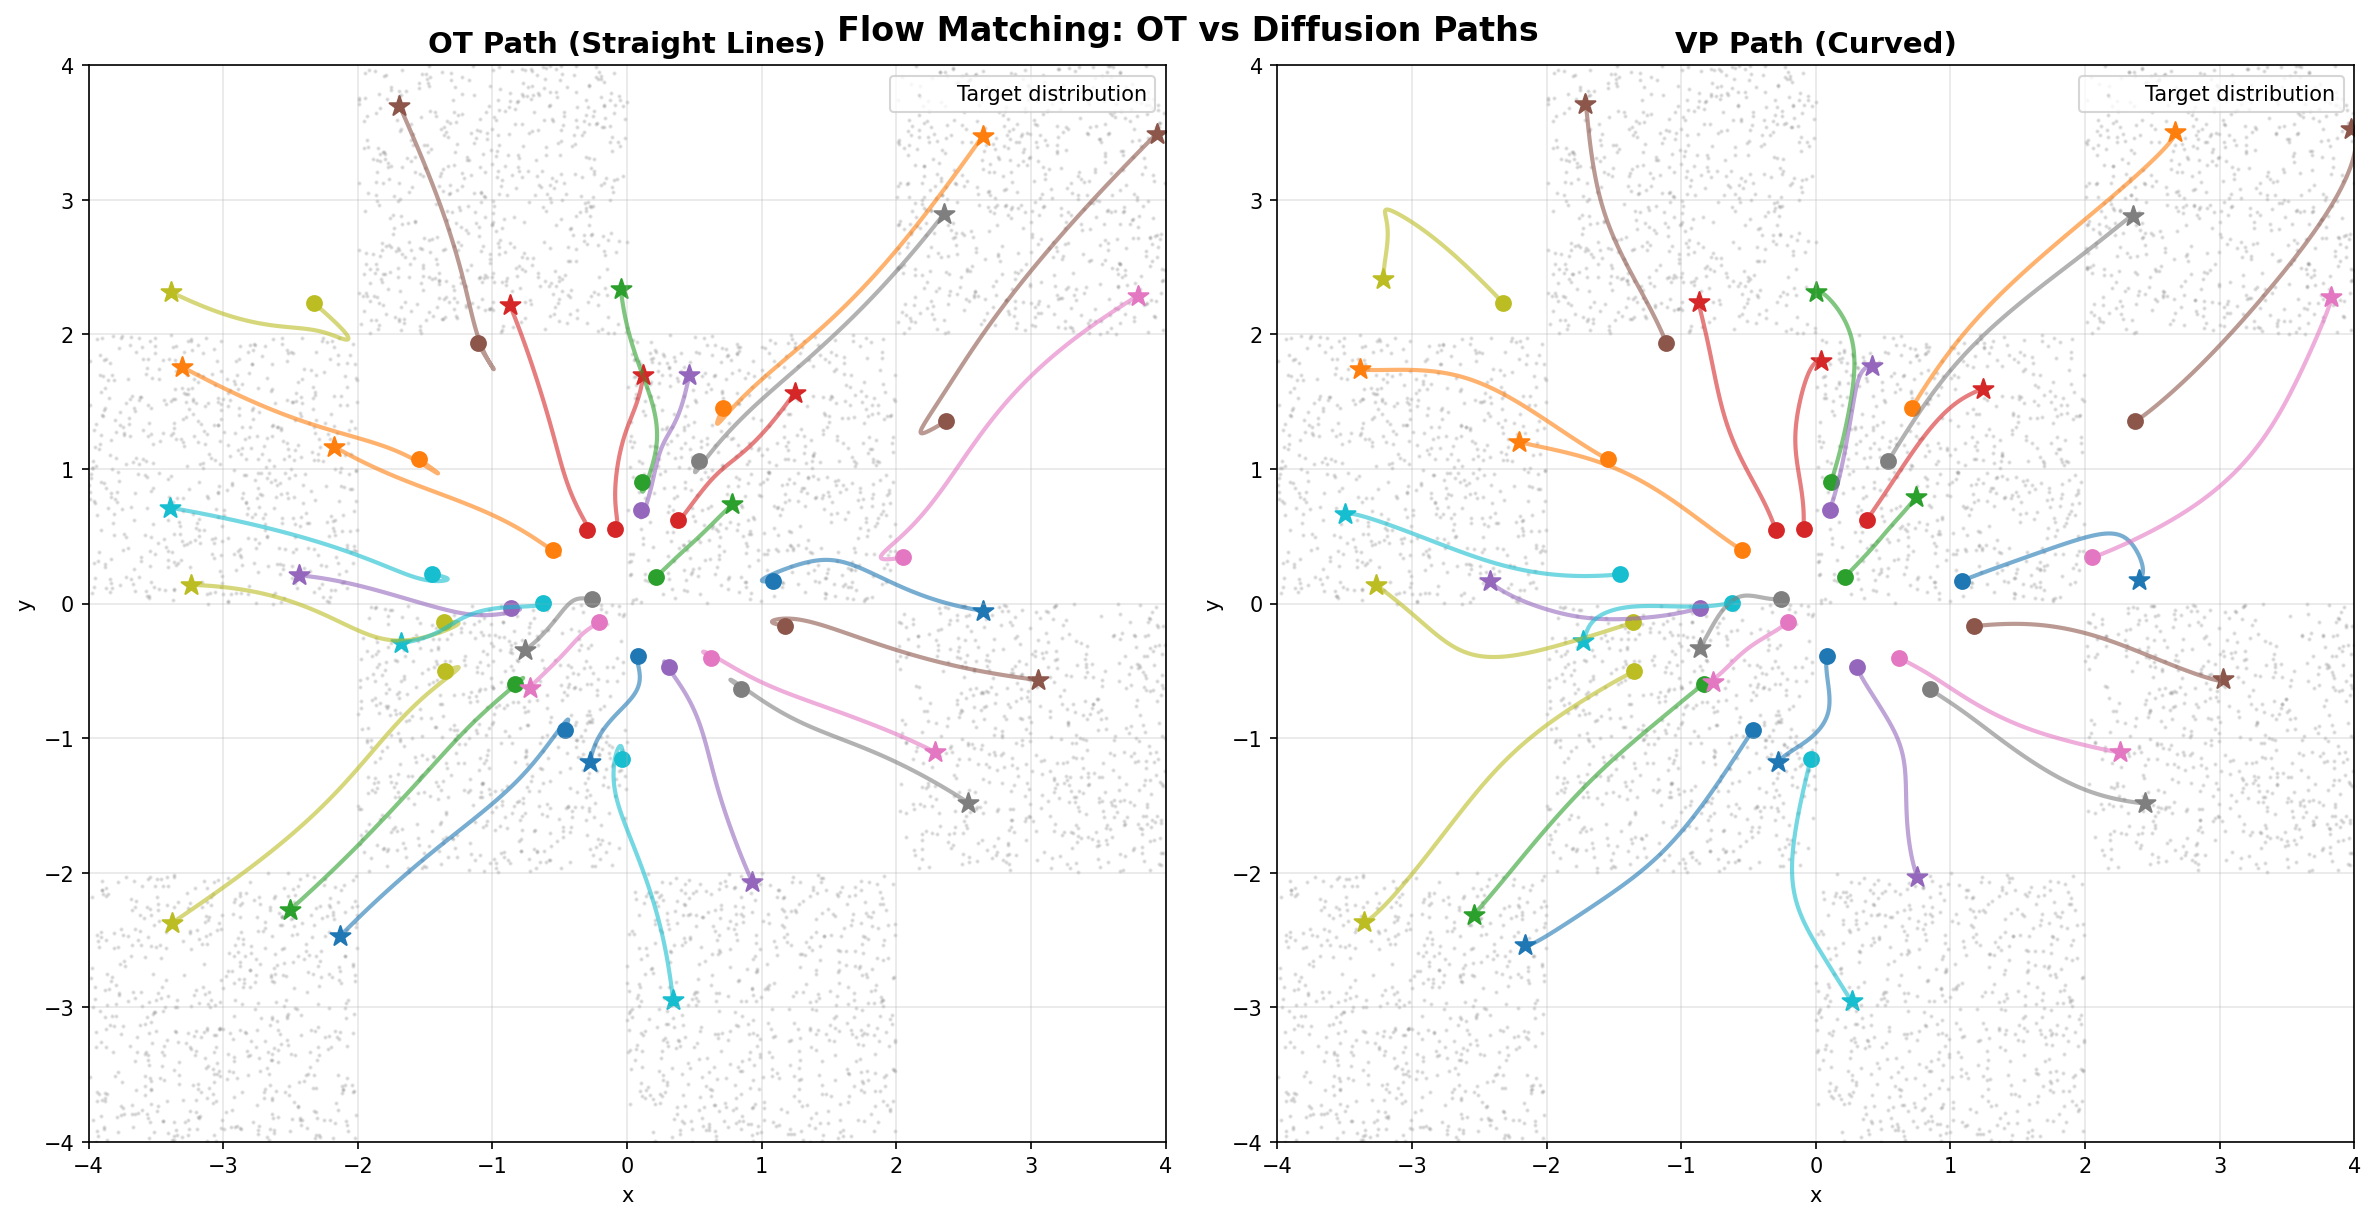
\includegraphics[width=\linewidth]{figures/toy/ot_vs_vp_trajectories.png}
    \caption{生成轨迹对比：OT（左）vs VP（右）}
    \label{fig:traj_compare}
\end{subfigure}
\begin{subfigure}{1\textwidth}
    \centering
    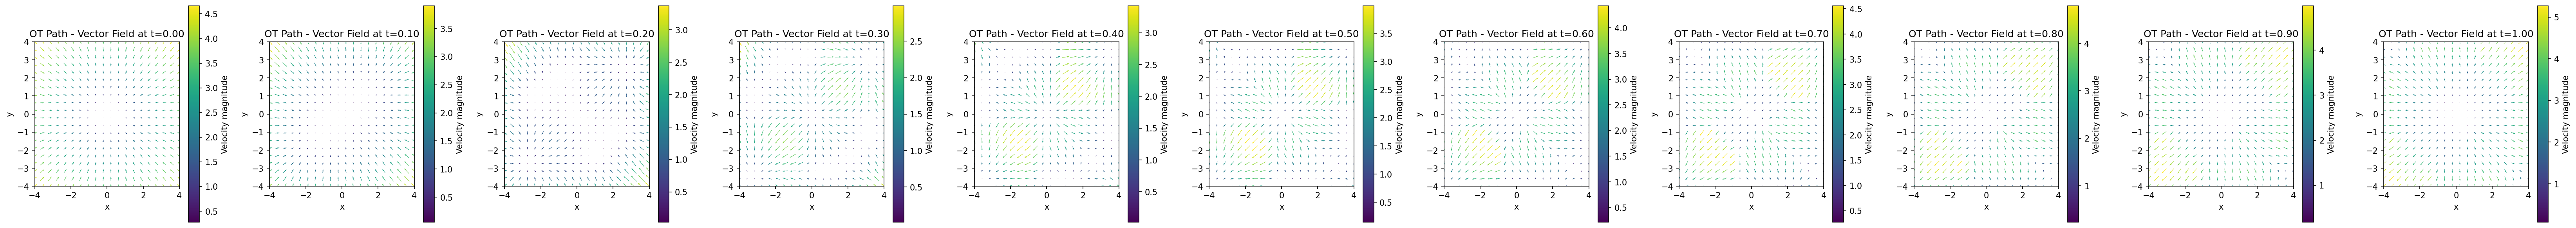
\includegraphics[width=\linewidth]{figures/toy/vector_field_OT.png}
    \caption{OT 向量场 ($t=0-1$)}
    \label{fig:vf_ot}
\end{subfigure}

\begin{subfigure}{1\textwidth}
    \centering
    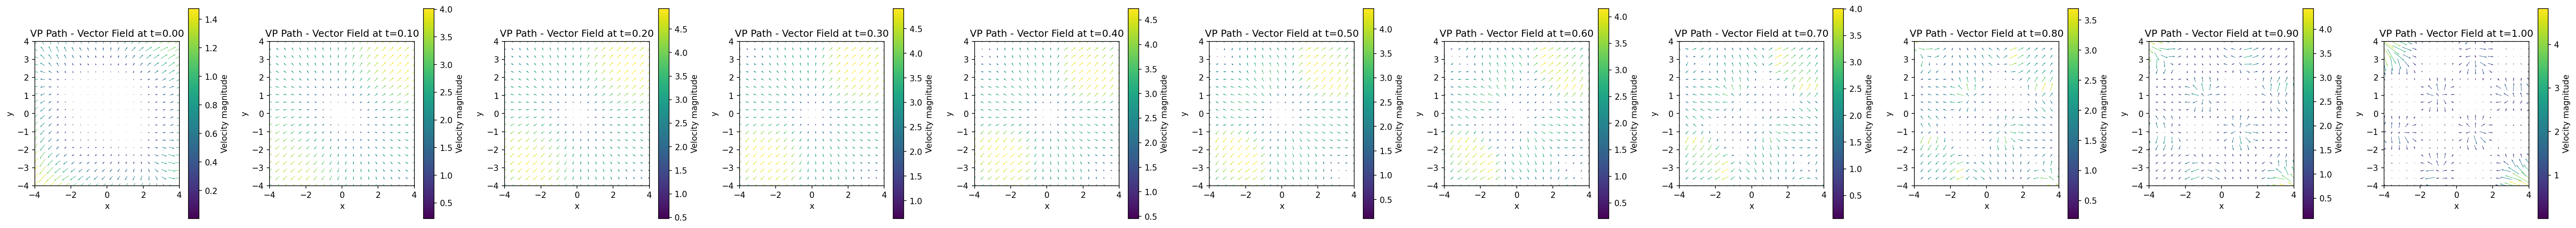
\includegraphics[width=\linewidth]{figures/toy/vector_field_VP.png}
    \caption{VP 向量场 ($t=0-1$)}
    \label{fig:vf_vp}
\end{subfigure}
\caption{微观机制分析。\textbf{(a)} 对于同一Flow过程，OT的曲线要比VP更直。\textbf{(b)-(c)} OT 向量场呈现出整齐的一致性方向，易于神经网络拟合；相比之下，VP 向量场包含复杂的旋转分量，学习难度更大。}
\label{fig:toy_mechanisms}
\end{figure}
\begin{enumerate}
    \item \textbf{轨迹直线性}：OT 路径生成的轨迹在几何上接近连接噪声分布与数据流形的直线。这意味着 ODE 求解器可以用极大的步长进行积分而不产生显著的截断误差。
    \item \textbf{向量场简单性}：OT 向量场在空间上变化平缓，方向一致性强。相比之下，VP 路径（以及传统的DDPM）对应的向量场往往包含旋转和非线性变化，需要更深的网络和更多的采样步数来精确捕捉。
\end{enumerate}

\subsection{CIFAR-10 采样效率分析}

本节通过 FID 随 NFE 变化的曲线（图 \ref{fig:nfe_comparison}）量化评估采样效率。

\begin{figure}[htbp]
\centering
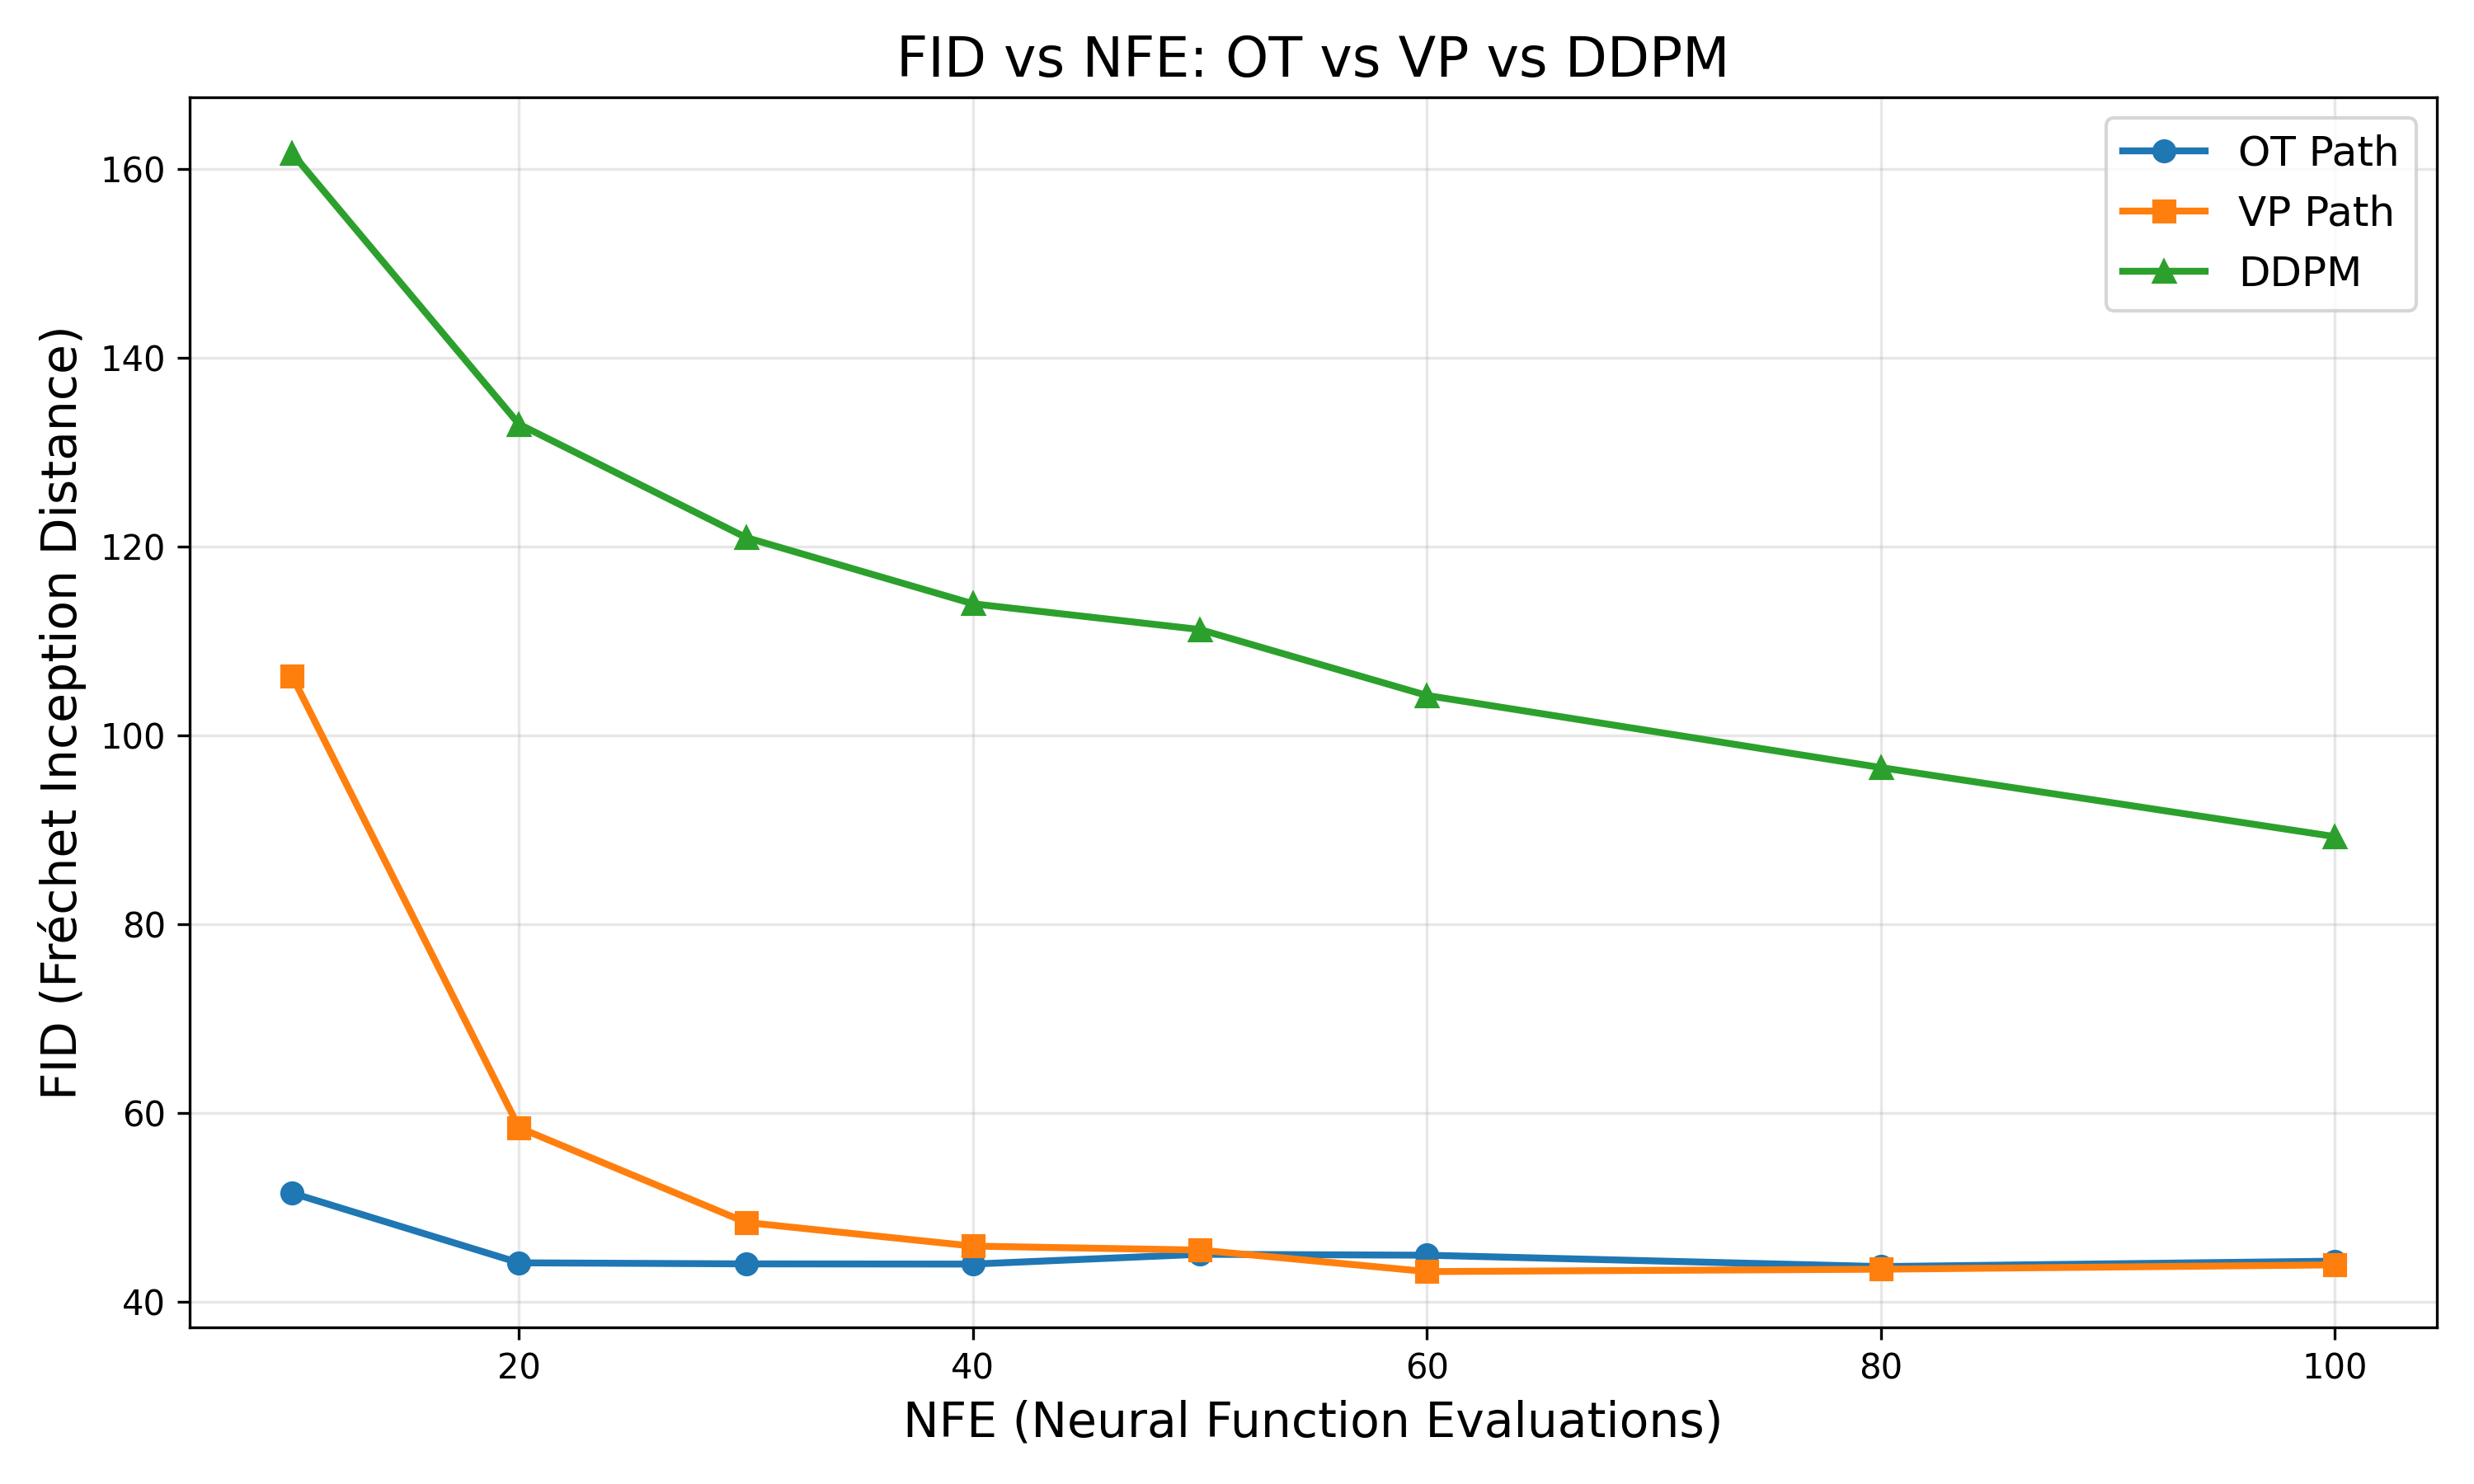
\includegraphics[width=0.6\textwidth]{figures/cifar10/nfe_comparison_three_way.png}
\caption{FID vs NFE 核心结果对比。OT 路径在极低步数下即可实现极高质量生成。}
\label{fig:nfe_comparison}
\end{figure}

\begin{table}[htbp]
\centering
\caption{不同步数下的 FID 性能对比（仅部分，测试样本数 2000）}
\label{tab:fid_comparison}
\begin{tabular}{l|cccc|c}
\hline
Method & FID@10 & FID@20 & FID@50 & FID@100 & Best FID \\
\hline
FM-OT  & \textbf{51.54} & \textbf{44.16} & \textbf{44.02} & 44.33 & 43.76 \\
FM-VP  & 106.28 & 58.47 & 45.92 & \textbf{43.93} & 43.23 \\
DDPM   & 161.65 & 132.95 & 113.94 & 89.28 & 89.28 \\
\hline
\end{tabular}
\end{table}

\begin{itemize}
    \item \textbf{效率优势}：在 NFE=10 时，FM-OT 的 FID已远超 NFE=100 时的 DDPM，实现极大的理论采样加速。
    \item \textbf{收敛稳定性}：OT 路径的 FID 随 NFE 增加表现出极强的稳定性，说明其对步长选取不敏感，这得益于其常数速度向量场的特性。
    \item \textbf{模型性能}：虽然受到优化与模型设计的细节问题，绝对 FID 高于原论文，但是能够看出相对趋势与论文一致，验证了 OT 路径在采样效率上的优势。
\end{itemize}

\subsection{类别定向生成结果}

通过引入 Cross-Attention 机制，模型成功实现了对 CIFAR-10 十个类别的定向生成。图 \ref{fig:class_conditional} 展示了随机选取的五个类别的生成结果。

\begin{figure}[htbp]
\centering
\begin{subfigure}{0.19\textwidth}
    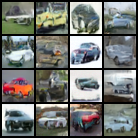
\includegraphics[width=\linewidth]{figures/cifar10/conditional/class_1.png}
    \caption{Car}
\end{subfigure}
\hfill
\begin{subfigure}{0.19\textwidth}
    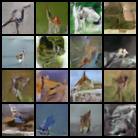
\includegraphics[width=\linewidth]{figures/cifar10/conditional/class_2.png}
    \caption{Bird}
\end{subfigure}
\hfill
\begin{subfigure}{0.19\textwidth}
    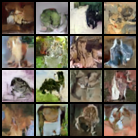
\includegraphics[width=\linewidth]{figures/cifar10/conditional/class_3.png}
    \caption{Cat}
\end{subfigure}
\hfill
\begin{subfigure}{0.19\textwidth}
    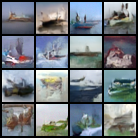
\includegraphics[width=\linewidth]{figures/cifar10/conditional/class_8.png}
    \caption{Ship}
\end{subfigure}
\hfill
\begin{subfigure}{0.19\textwidth}
    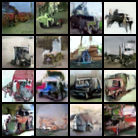
\includegraphics[width=\linewidth]{figures/cifar10/conditional/class_9.png}
    \caption{Truck}
\end{subfigure}
\caption{类别定向生成样本展示。模型能够准确根据输入标签生成具有对应语义特征的图像，证明了 Flow Matching 框架在条件生成任务中的有效性。}
\label{fig:class_conditional}
\end{figure}

实验表明，基于 OT 路径的 Flow Matching 配合交叉注意力机制，即便在较小的参数量（2.4M）下，也能产生具有清晰轮廓和正确语义的样本。这进一步验证了向量场回归在处理复杂条件分布时的灵活性。

\section{结论}
\label{sec:conclusion}

本文基本复现了Flow Matching论文的核心实验，在2D Toy数据和CIFAR-10数据集上验证了最优传输（OT）路径的优势。通过完整实现OT、VP、DDPM三种方法并进行系统对比，我们发现：

\begin{enumerate}
\item OT路径在低NFE下显著优于VP路径和DDPM；
\item Flow Matching训练更简单，无需复杂的beta schedule设计；
\item 向量场可视化验证了理论：OT路径的方向一致，易于学习；VP路径有旋度，模式复杂
\item 实验结果的相对趋势与Flow Matching论文一致，验证了OT路径在采样效率上的优势
\end{enumerate}



\bibliographystyle{IEEEtran}
\bibliography{references}
%后注：
\textbf{AI使用情况说明}：
报告写作的过程中使用了gemini与copilot，但是由于这个实验项目相对较为复杂，
仅实验结果就有数百张图像，所以gemini主要用于基本的latex的框架搭建与
语言润色，copilot主要用于tabletabletable进行一部分补全，
实验结果与分析均为本人独立完成。
\end{document}